\documentclass[letterpaper,12pt]{article}

\usepackage[margin=1in]{geometry}
\usepackage{titling}
\usepackage{graphicx}

\setlength{\droptitle}{-0.75in}

\title{Fault Tolerance in Block-Level Caching}
\author{
  Jesus Ramos \\ \texttt{jramo028@fiu.edu} \and
  Douglas Otstott \\ \texttt{dotst001@fiu.edu}
}
\date{}

\pagestyle{empty}

\begin{document}

\maketitle
\thispagestyle{empty}

\section*{Problem Statement}

Many companies are switching to warehouse scale computing to deal with
increasing computing demands due to the cost and efficiency of
warehouse architecture. Rather than trying to prevent failure, most
warehouse scale computing solutions accept failure and attempt to
integrate recovery as seamlessly as possible\cite{Placeholder}.
\\ \\*
%
Dependability and reliability are two important factors when dealing
with cloud and warehouse scale computing. Systems should be robust and
be able to recover from errors and failure effectively and quickly.
\\ \\*
%
Fault tolerance is still a major issue in cloud based systems that
employ caching. Currently in the event of an error or power failure
all data that was pending to be written back is lost along with
currently cached data. In some cases minor data loss is acceptable,
but in most cases even minor loss of data can result in larger
problems and error recovery can become very complex depending on the
type and quantity of data lost.

% end section Problem Statement

\section*{Problem Background}

\begin{center}
  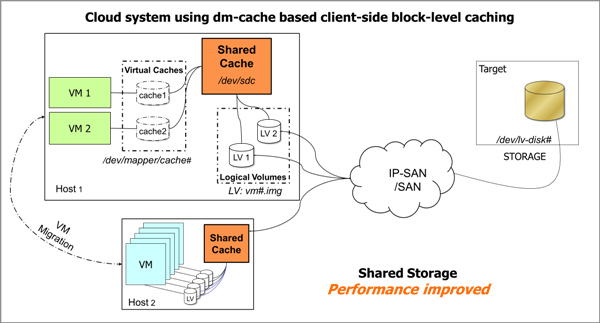
\includegraphics{../Images/NewerImage.png}
\end{center}
\noindent
Many large scale cloud based systems employ network storage due to the
physical limitations of local storage devices. Basically, each host
machine in the cloud is connected to a small number of machines which
are responsible for all persistent data management across the system.
These machines create what is known as a Storage Area Network (SAN).
SAN's are a common solution used by cloud service providers due to the
simplification of virtual machine migration and increased data
reliability. While this solves the storage size problem it also
increases the response latency and creates a bandwidth issue due to
the sheer volume of requests constantly sent to the storage devices.
\\ \\*
%
Local caches are employed by many systems as a means to bring in the
most frequently used data to more local storage devices to reduce
latency and alleviate pressure on the main storage system. DM-Cache is
an open-source block-level caching solution developed as a Linux
kernel module. DM-Cache allows host machines to store the most
recently used blocks in a designated storage device. Preliminary
testing on DM-Cache indicates a significant improvement in systems
where numerous hosts and virtual machines create a bottleneck in terms
of network storage bandwidth. However, local caching introduces a new
problem in terms of fault tolerance as locally modified blocks are lost
in the event of system failure.

% end section Problem Background

\section*{Proposed Solution}

Our proposed solution is to add functionality to DM-Cache to allow
persisting of the cache meta data to the disk. This meta data can then
be used in case of power or system failure and will minimize the data
lost in the event of a system failure.
\\ \\*
%
This solution can also provide for quicker recovery time in the event
of an error as we can use the meta data that was persisted to

% end section Proposed Solution

\section*{Project Timeline}

The first phase of this project is to do some research on methods for
persisting cache meta-data effectively so that recovery can be done
quickly and efficiently when the cache is being recreated.
\\ \\*
%
Once we have decided on the method for persisting the data we will
actually implement this into DM-Cache and add an option when creating
the cache to allow for recovery of the previous cache in case of
system failure.
\\ \\*
%
The last phase will involve testing and evaluation of just how robust
the system will be in the even of a system failure such as power or
system crash.

% end section Project Timeline

\section*{Project Evaluation}

Test citation and placeholder for project evaluation \cite{Test}

% end section Project Evaluation

% Bibtex section

\bibliography{proposal}
\bibliographystyle{plain}

\end{document}
